% Intended LaTeX compiler: pdflatex
\documentclass[10pt,a4paper,UTF8]{article}
\usepackage{zclorg}
\author{张朝龙}
\date{}
\title{不变子空间}
\hypersetup{
 pdfauthor={张朝龙},
 pdftitle={不变子空间},
 pdfkeywords={},
 pdfsubject={},
 pdfcreator={Emacs 25.0.50.1 (Org mode 9.0.5)},
 pdflang={English}}
\begin{document}

\maketitle
\tableofcontents
\titlepic{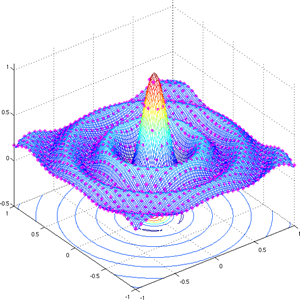
\includegraphics[scale=0.25]{../../img/sinc.PNG}}

\section{回忆}
\label{sec:org358e2b0}


\href{invertible-isomorphic.org}{算子} 是从一个向量空间到自身的线性映射。\(V\)上的算子集合记为\(\mathcal{L}(V)\)。为了更好的理解算子,假设\(T\in \mathcal{L}(V)\),如果\(V\)有直和分解:\[V  = U_{1} \oplus \ldots \oplus U_{m}\] 其中\(U_{j},j\in \{1,\ldots ,m\}\)是\(V\)的真子空间,那么,如果想要了解\(T\)的特性,我们只需要了解每个\(T|_{U_{j}}\)的特性就可以了。这里\(T|_{U_{j}}\)表示把\(T\)限制到更小的定义域\(U_{j}\)上。因为\(U_{j}\)是比\(V\)更小的向量空间,所以处理\(T|_{U_{j}}\)应该比\(T\)更容易。

但是这里有个问题:\(T|_{U_{j}}\)是\(U_{j}\)上的算子么?显然,不一定的。那么为了进一步简化分析,我们只考虑那些\(T\)能够把\(U_{j}\)映射到\(U_{j}\)的直和分解,即在这样的直和分解结果中\(T|_{U_{j}}\)依然是\(U_{j}\)上的算子。

\section{被算子映射到自身的子空间}
\label{sec:orgce61769}


被算子映射到自身的子空间非常重要。因此我们赋予它一个名字:
\begin{definition}
设\(T\in \mathcal{L}(V)\),称\(V\)的子空间\(U\)在\(T\)下不变,如果对于每个\(u\in U\)都有\(Tu \in U\)
\end{definition}

\begin{instance}
设\(T\in \mathcal{L}(V)\),证明\(V\)的下列子空间在\(T\)下不变:
\begin{enumerate}
\item \(\{0\}\)
\item \(V\)
\item \(nullT\)
\item \(rangeT\)
\end{enumerate}
\end{instance}

\begin{proof}
\begin{enumerate}
\item 对于\(\{0\}\)中的元素\(0\),\(T(0) = 0 \in \{0\}\)
\item 对于\(V\), \(\forall v\in V, T(v) \in V\),因为\(T\)是\(V\)上的算子。
\item 对于\(nullT\), \(\forall u \in nullT\), \(Tu = 0 \in nullT\)
\item 对于\(rangeT\),\(\forall u \in rangeT\),\(Tu \in rangeT\)
\end{enumerate}
\end{proof}

这四个空间是\(V\)的固有的四个不变子空间。

\section{本征值与本证向量}
\label{sec:org0373068}


不变子空间的研究可以非常深入,泛函分析中,最终名的尚未解决的问题叫做 \textbf{不变子空间问题} , 它研究无限维向量空间上算子的不变子空间。现在我们先研究最简单的非平凡不变子空间:一维不变子空间。

\(\forall v\in V, v\neq 0\),并设\(U\)是\(v\)的标量倍构成的集合:\[U = \{\lambda v: \lambda \in \mathbf{F}\} = span(v) \]
则,\(U\)是\(V\)的一维子空间。若\(U\)在算子\(T\in \mathcal{L}(V)\)下不变,则\(Tv\in U\),因此必有标量\(\lambda\in \mathbf{F}\)使得\(Tv = \lambda v\)

另一方面,若有某个\(\lambda \in \mathbf{F}\)使得\(Tv = \lambda v\),则\(span(v)\)是\(V\)的在\(T\)下不变的一维子空间。终于,我们现在见到了本征值和本证向量。这种引入方式不同于生硬的定义,深入浅出的谆谆善诱。在使用《linear algebra done right》这本书的时候,恨不得把自己的大脑格式化一遍,从新学习线性代数。之前学的东西忘不掉,又不成体系,只发挥了扰乱心智的作用。

\begin{definition}
设\(T\in \mathcal{L}(V)\),称数\(\lambda \in \mathbf{F}\)为\(T\)的本征值,若存在\(v\in V,v\neq 0\),使得\(Tv = \lambda v\)
\end{definition}

小插曲: \textbf{eigenvalue} 这个词一半是德文,一半是英文。德文形容词 \textbf{eigen} 的意思是 “特有的”。有些数学家使用特征值而不是本征值。我学线性代数的时候使用特征值这种说法。

本征值的等价条件:设\(V\)是有限维的,\(T\in \mathcal{L}(V)\),且\(\lambda\in \mathbf{F}\),\(I\)是恒等映射,则以下条件等价:
\begin{enumerate}
\item \(\lambda\)是\(T\)的本征值;
\item \(T-\lambda I\)不是单的;
\item \(T-\lambda I\)不是满的;
\item \(T-\lambda I\)不是可逆的。
\end{enumerate}

我们之前就证明过一个命题:对于有限维空间,现行算子的单性,满性和可逆性是等价的, 见\href{invertible-isomorphic.org}{这里} 。

\begin{definition}
设\(T\in \mathcal{L}(V)\),并设\(\lambda \in \mathbf{F}\)是\(T\)的本征值,称向量\(v\in V\)为\(T\)的相应于\(\lambda\)的本徵向量,如果\(v\neq 0\)且\(Tv = \lambda v\)
\end{definition}

因为\(Tv = \lambda v\)当且仅当\((T - \lambda I)v = 0\),说明\(v\in null(T-\lambda I)\)

\begin{theorem}
设\(T\in \mathcal{L}(V)\),设\(\lambda_{1},\ldots ,\lambda_{m}\)是\(T\)的互不相同的本征值,并设\(v_{1},\ldots ,v_{m}\)是相应的本证向量,则\(v_{1},\ldots ,v_{m}\)是线性无关的。
\end{theorem}

\begin{proof}
采用反证法。设\(v_{1},\ldots ,v_{m}\)是线性相关的,我们希望能够推出矛盾。假设\(k\)是满足\(k\in span(v_{1},\ldots ,v_{k-1})\)成立的最小正整数。根据线性相关引理,这个正整数是存在的,并且\(v_{1},\ldots ,v_{k-1}\)是线性无关的(因为任何小于\(k\)的数都不能是\(v_{k}\in span(v_{1},\ldots ,v_{k-1})\),根据线性无关的定义,我们知道\(v_{1},\ldots ,v_{k-1}\)是线性无关的)。

因为\(v_{k}\in span(v_{1},\ldots ,v_{k-1})\),所以\[\exists a_{1},\ldots ,a_{k-1}, \quad v_{k} = a_{1}v_{1} + \ldots + a_{k-1}v_{k-1} \]我们对上式分别做两个操作:
\begin{enumerate}
\item 乘以\(\lambda_{k}\)
\item 执行\(T\)映射
\end{enumerate}
我们会得到两个式子:
\begin{eqnarray}
\label{eq:1}
\lambda_{k}v_{k}&=& \lambda_{k}a_{1}v_{1} + \ldots + \lambda_{k}a_{k-1}v_{k-1} \\
\lambda_{k}v_{k}&=& \lambda_{1}a_{1}v_{1} + \ldots + \lambda_{k-1}a_{k-1}v_{k-1}
\end{eqnarray}
两式相减则有:
\begin{equation}
\label{eq:2}
0 = a_{1}(\lambda_{k} - \lambda_{1}) v_{1} + \ldots + a_{k-1}(\lambda_{k} - \lambda_{k-1})v_{k-1}
\end{equation}

因为\(v_{1},\ldots ,v_{k-1}\)是线性无关的,所以:
\begin{eqnarray*}
a_{1}(\lambda_{k} - \lambda_{1})&=&0 \\
\vdots &=& \vdots \\
a_{1}(\lambda_{k} - \lambda_{k-1})&=&0
\end{eqnarray*}
因为\(\lambda_{k}\)不与\(\lambda_{1},\ldots ,\lambda_{k-1}\)中的任何一个相等,所以\(a_{j}=0,\forall j\)。所以\(v_{k} = 0\)这与\(v_{k}\)是本证向量的假设矛盾。

所以\(v_{1},\ldots ,v_{m}\)都是线性无关的。
\end{proof}
这个定理的证明依赖于线性相关性引理,现在把这个引理复数如下:
\begin{theorem}
设\(v_{1},\ldots ,v_{m}\)是\(V\)中的一个线性相关的向量组,则有\(j\in \{1,\ldots ,m\}\)使得:
\begin{enumerate}
\item \(v_{j}\in span(v_{1},\ldots ,v_{j-1})\)
\item 若从\(v_{1},\ldots ,v_{m}\)中去掉第\(j\)项,则剩余组的张成空间等于\(span(v_{1},\ldots ,v_{m})\)
\end{enumerate}
\end{theorem}
结合线性相关性引理的两个步骤,我们可以迭代的找到那个使得\(v_{1},\ldots ,v_{j}\)线性无关的\(k\),即\(v_{1},\ldots ,v_{k}\)是线性无关的,但是\(v_{1},\ldots ,v_{k+1}\)是线性相关的,且\(v_{k+1}\in span(v_{1},\ldots ,v_{k})\)。

\begin{theorem}
设\(V\)是有限维的,则\(V\)上的每个算子最多有\(\dim V\)个互不相同的本征值。
\end{theorem}

\begin{proof}
设\(T\in \mathcal{L}(V)\),设\(\lambda_{1},\ldots ,\lambda_{m}\)是\(T\)的互不相同的本征值,\(v_{1},\ldots ,v_{m}\)是相应的本证向量。由于\(v_{1},\ldots ,v_{m}\)是线性无关的,所以\(m \leq \dim V\)。一个向量空间中的线性无关组的长度小于这个向量的基中向量组的长度。
\end{proof}
\section{限制算子与商算子}
\label{sec:org2fee96f}


若\(T\in \mathcal{L}(V)\)且\(U\)是\(V\)的在\(T\)下不变的子空间,则\(U\)默认定了另外两个算子\(T|_{U} \in \mathcal{L}(U)\),和\(T/U \in \mathcal{L}(V/U)\),其定义为:
\begin{definition}
设\(T\in \mathcal{L}(V)\),且\(U\)是\(V\)的在\(T\)下不变的子空间。
\begin{enumerate}
\item 限制算子 \(T|_{U} \in \mathcal{L}(U)\)的定义为:\[\forall u\in U, T|_{U}(u) = Tu\]
\item 商算子\(T/U \in \mathcal{L}(V/U)\)定义为:\(\forall v\in V, (T/U)(v+U) = Tv + U\)
\end{enumerate}
\end{definition}

首先考虑限制算子\(T|_{U}\in \mathcal{L}(U)\)这个算子之所以叫限制算子,是因为这个算子把映射的定义域限制在\(U\)上。并且\(T|_{U}\)是把\(U\)上的元素映射到\(U\)上而不是\(V\)上。

对于商算子,我们需要验证\(v+U = w +U\),则\(Tv + U = Tw + U\)。现在设\(v+U = w+U\),则\(v-w \in U\)。由于\(U\)在\(T\)下不变,则\(T(v-w)\in U\),即\(Tv - Tw\in U\),所以\(Tv + U = Tw + U\)。

设\(T\)是有限维向量空间\(V\)上的算子,且\(U\)是\(V\)在\(T\)不变的子空间使得\(U\neq \{0\}\)且\(U\neq V\)。在某种意义下,可以通过研究算子\(T|_{U}\)和\(T/U\)来了解算子\(T\),而\(T|_{U}\)和\(T/U\)都是维数小于\(V\)维数的向量空间上的算子。但是,有时候\(T|_{U}\)和\(T/U\)并没有给出关于\(T\)的足够信息。在下面的例子中,\(T|_{U}\)和\(T/U\)都是\(0\),即便\(T\)不是\(0\)算子。

\begin{instance}
定义算子\(T\in \mathcal{L}(\mathbf{F}^{2})\)为\(T(x,y) = (y,0)\),设\(U=\{(x,0):x\in \mathbf{F}\}\)。证明:
\begin{enumerate}
\item \(U\)在\(T\)下不变。且\(T|_{U}\)是\(U\)上的\(0\)算子。
\item 不存在\(\mathbf{F}^{2}\)的在\(T\)下不变的子空间\(W\)使得\(\mathbf{F}^{2} = U\oplus W\)
\item \(T/U\)是\(\mathbf{F}^{2}/U\)上的\(0\)算子
\end{enumerate}
\end{instance}

\begin{proof}
\begin{enumerate}
\item 对于\((x,0)\in U\),我们有\(T(x,0) = (0,0)\in U\),所以\(T|_{U}\)在\(U\)下不变,且\(T|_{U}\)是\(U\)的\(0\)算子。
\item 设\(W\)是\(V\)的子空间使得\(\mathbf{F}^{2} = U\oplus W\),由于\(\dim \mathbf{F}^{2} = 2\)且\(\dim U = 1\),我们有\(\dim W = 1\)。若\(W\)在\(T\)下不变,则\(W\)的每个非零向量都是\(T\)的本证向量。然而\(T\)的唯一本征值是\(0\),且\(T\)的所有本证向量都在\(U\)中。于是\(W\)并非在\(T\)下不变。
\item 对于\((x,y)\in \mathbf{F}^{2}\),我们有:
\end{enumerate}
\[(T/U)((x,y) + U) = T(x,y) + U = (y,0) + U = U\]
因为\(U\in V/U\),且是\(V/U\)里的单位元,所以\(T/U\)是\(0\)算子。
\end{proof}
\end{document}
